
\documentclass[a4paper,oneside,titlepage,11pt]{report}

%\includeonly{acknowledgements,abbreviations,introduction,eng_review,opt_review,lin_elast_finite_elements,min_comp_st_vol,buckling,analysis_eso,conclusion,appendix}
%\includeonly{buckling,eng_review,opt_review,analysis_eso}
%\includeonly{min_comp_st_vol}
%\includeonly{acknowledgements}
%\includeonly{eng_review}

% this includes the baththesis package
\usepackage{readingthesis}
%\usepackage[latin1]{inputenc}
\usepackage{amsmath,amssymb,amsthm}%,amsxtra}
\usepackage{graphicx}
\usepackage{fancyhdr}   % does nice headers (not required)
%\usepackage{subfig}
%\usepackage{caption}
%\usepackage{subcaption}
%\usepackage[notref,notcite]{showkeys}
%\usepackage{multibib}
%\usepackage{float}
\usepackage{tikz}
\usepackage{tikz-3dplot}
\usetikzlibrary{shapes.geometric,arrows,automata,positioning}
\usepackage{nomencl}
\makenomenclature
\usepackage[Glenn]{fncychap}
%\usepackage[margin=0pt,font=small,labelfont=bf,textfont=it]{caption}

%\usepackage{makeidx}	       % this package makes an index - it is not required!
%\makeindex
\usepackage[pdftex,pdfborder= 0 0 0,citecolor=black,linkcolor=black,colorlinks=true,bookmarksopen=true,plainpages=false,pdfpagelabels]{hyperref}
\pagestyle{fancy}
%\usepackage{algorithm}	% those two packages are helpful if you use a lot of algorithms in your thesis
%\usepackage{algorithmic} 
\usepackage{tabularx}
\usepackage{ifthen}
\usepackage{pgf}
\usepackage{pgfplots}
\usepackage{datetime}

% From Dan Peak's thesis:
%\usepackage{lscape}
%,latexsym,flafter,afterpage,amssymb}
%\usepackage[round]{natbib}
%\usepackage{setspace}
%\onehalfspacing
%\usepackage[font=singlespacing,small,bf]{caption}
%\usepackage[small,bf]{caption}
\usepackage{array}
\usepackage{subfigure} %, epsfig, amsmath,multirow,lscape}
\usepackage{graphicx}
%\usepackage{latexsym,flafter,afterpage,amssymb,color}
%\usepackage[round]{natbibnew}
\usepackage{natbib}
%\usepackage{amssymb,amsmath}
%\usepackage{subfigure}
%\usepackage{amsthm}
\usepackage{lineno}
\usepackage{colortbl}
%\usepackage{tikz}
%\usepackage{pgfplots}
\usepgfplotslibrary{colormaps,external}
\usepackage{pgfkeys}
\usetikzlibrary{calc,intersections,through,backgrounds,decorations.pathmorphing,decorations.pathreplacing, decorations.shapes}
\usepackage{wrapfig}
%\usepackage{float}
\usepackage{comment}
\usepackage{placeins}


\theoremstyle{plain}

\newtheorem{thm}{Theorem}[chapter]		% those commands are for numbering Theorems etc within the chapter
\newtheorem{Example}[thm]{Example}
\newtheorem{lemma}[thm]{Lemma}
\newtheorem{defn}[thm]{Definition}
\newtheorem{Remark}[thm]{Remark}
\newtheorem{cor}[thm]{Corollary}
\newtheorem{prop}[thm]{Proposition}
\newtheorem{algo}[thm]{Algorithm}
\newtheorem{Assumption}[thm]{Assumption}
\newtheorem{Conjecture}[thm]{Conjecture}



\newcommand{\D}[2]{\frac{\partial #1}{\partial #2}}
\newcommand{\bs}{\boldsymbol}
\newcommand{\pd}{\partial}
\newcommand{\var}{\operatorname{Var}}
\newcommand{\cov}{\operatorname{Cov}}
% headings 

\renewcommand{\headrulewidth}{1pt}
\renewcommand{\footrulewidth}{1pt}

\fancyhead[EL,OL]{}
\fancyhead[ER]{\sffamily\footnotesize\nouppercase{\rightmark}}
\fancyhead[OR]{\sffamily\footnotesize\nouppercase{\leftmark}}

\fancyfoot[EL,OR]{}
\fancyfoot[EC,OC]{\sffamily\thepage}

% spacing, choose whatever you want - the university regulations say single or onehalfspacing is okay, 
% the default is single spacing

\doublespacing
%\onehalfspacing
%\linespread{1.1}

% this is the title, obviously

\title{\sffamily\bfseries Understanding the information content in diverse observations of carbon stocks and fluxes for data assimilation and ecological modelling} 
\author{\sffamily Ewan Mark Pinnington}
\degree{\sffamily Doctor of Philosophy}
\department{\sffamily Department of Meteorology}
\degreemonthyear{\sffamily \monthname \ \the\year} \norestrictions
\makeatletter \AtBeginDocument{	\hypersetup{pdftitle= {\@title \ - E. Pinnington PhD Thesis, University of Reading},pdfauthor= {\@author}}} \makeatother




%\rfoot{
%{\setlength{\unitlength}{1mm}\begin{picture}(0,0)\put(0,-33){\includegraphics[width=2cm]{/home/pab23/2012/apple/pics/\thepage.jpg}}\end{picture}}
%}

\fancypagestyle{plain}{%
\fancyhf{}
\renewcommand{\headrulewidth}{0pt}
\renewcommand{\footrulewidth}{0pt}
%\fancyfoot[EC,OC]{\sffamily\thepage}
%\rfoot{
%{\setlength{\unitlength}{1mm}\begin{picture}(0,0)\put(0,-33){\includegraphics[width=2cm]{/home/pab23/2012/apple/pics/\thepage.jpg}}\end{picture}}
} %}

\begin{document}
\maketitle
\clearpage

\chapter*{Declaration}
%%\chapter*{\vspace*{5pt}\centering \scshape Abstract}
%\thispagestyle{headings}
%%\thispagestyle{contents}%%

\par
I confirm that this is my own work and the use of all material from
other sources has been properly and fully acknowledged.

\vspace*{1cm}
\hspace{3.75in} M. S. Lang

\newpage
%\thispagestyle{empty}
%\hspace{1cm}
%\clearpage

% acknowledgements, in case you want to include them
%\thispagestyle{empty}

\pagenumbering{roman}
\begin{abstract}
%\chapter*{\centering \Large \vspace{-20mm}\Huge Abstract}

%=========================================================
%Abstract goes here

%Forests and terrestrial ecosystems play an important role in the global carbon cycle, removing large amounts of CO\(_2\) from the atmosphere and thus helping to mitigate the effect of human-induced climate change. Land surface carbon uptake is the most uncertain process in current estimates of the global carbon cycle. There is much disagreement on whether forests and terrestrial ecosystems will continue to remove the same percentage of CO\(_2\) from the atmosphere under future emission scenarios. It is therefore important to improve understanding of ecosystem carbon cycle processes in context of a changing climate. 

%In this talk we explore new techniques to improve estimates of ecosystem carbon uptake, with focus on the Alice Holt research forest in Hampshire. We then use these techniques, along with complimentary measurements obtained from an extensive fieldwork campaign, to better understand the effect of selective felling on the carbon dynamics of the Alice Holt forest. The response of ecosystem carbon uptake to land use change and disturbance (e.g. fire, felling, insect outbreak) is another large uncertainty in the global carbon cycle. Our methods represent a novel way to help elucidate this response. 

%In this talk we explore new techniques to improve estimates of ecosystem carbon uptake, with focus on the Alice Holt research forest in Hampshire. We then use these techniques, along with complimentary measurements obtained from an extensive fieldwork campaign, to better understand the effect of disturbance from selective felling on the carbon dynamics of the Alice Holt forest. Our methods represent a novel way to help elucidate the response of the forest to disturbance and changing climate.

%Forests play an important role in the global carbon cycle, removing large amounts of CO\(_2\) from the atmosphere and thus helping to mitigate the effect of human-induced climate change. The state of the global carbon cycle in the IPCC AR5 suggests that the land surface is the most uncertain component of the global carbon cycle.  The response of ecosystem carbon uptake to land use change and disturbance (e.g. fire, felling, insect outbreak) is a large component of this uncertainty. A main cause for the high level of uncertainty in terrestrial carbon balance predictions arise from significant gaps in current direct observations and poor parameterisations or missing processes in current modelled predictions. The mathematical technique of data assimilation presents a method for combing incomplete observational records with modelled predictions in order to find the best estimate for the state and parameter variables of a system. Data assimilation has risen to prominence in the field of numerical weather prediction where it has contributed to significant improvements in model forecasts. More recently data assimilation has been used to improve our knowledge of land surface carbon cycle processes. This field is still relatively new and underdeveloped in comparison with numerical weather prediction.

%In this thesis we aim to develop novel data assimilation techniques for the terrestrial carbon cycle. There are three main areas which we address; Understanding the information content in observations for data assimilation, Improving the characterisation of uncertainties in both prior model and observational estimates and using data assimilation to understand the effect of disturbance on the carbon dynamics of a managed woodland.

%It is important to understand which observations can add most information to data assimilation schemes so that choices for field campaigns can be made more sophisticatedly and the most uncertain components of land surface models constrained. In order to better understand information content and improve data assimilation results it is also imperative that we improve the characterisation and estimates of errors in our data assimilation schemes. Using these novel data assimilation techniques along with supplementary observations from a field work campaign we attempt to improve understanding of the effect of selective felling on forest carbon dynamics.         

%Additionally, there is much disagreement on whether forests and terrestrial ecosystems will continue to remove the same proportion of CO\(_2\) from the atmosphere under future climate regimes. It is therefore important to improve our understanding of ecosystem carbon cycle processes in the context of a changing climate.

Forests play an important role in the global carbon cycle, removing large amounts of CO\(_2\) from the atmosphere and thus helping to mitigate the effect of human-induced climate change. Land surface carbon uptake and its response to disturbance (e.g. fire, felling, insect outbreak) are the most uncertain component in the global carbon cycle. A main cause for the high level of uncertainty in terrestrial carbon balance predictions arise from significant gaps in current direct observations and poor parameterisations or missing processes in current modelled predictions. The mathematical technique of data assimilation presents a method for combing incomplete observational records with modelled predictions in order to find the best estimate for the state and parameter variables of a system. Data assimilation has risen to prominence in the field of numerical weather prediction where it has contributed to significant improvements in model forecasts. More recently data assimilation has been used to improve our knowledge of land surface carbon cycle processes. This field is still relatively new and underdeveloped in comparison with numerical weather prediction.

In this thesis we aim to develop novel data assimilation techniques for the terrestrial carbon cycle. There are three main areas which we address: understanding the information content in observations for data assimilation, improving the characterisation of uncertainties in both prior model and observational estimates and using data assimilation to understand the effect of disturbance on the carbon dynamics of a managed woodland. It is important to understand which observations add most information to data assimilation schemes in order to further understanding of unconstrained systems. We show how information content can vary temporally and with different characterisations of errors. We outline new representations of error for ecosystem carbon balance data assimilation schemes (specifically correlations between errors) and show how these can significantly improve data assimilation results. We then use these novel techniques in addition to supplementary observations obtained from a fieldwork campaign to investigate the effect of disturbance from selective felling on forest carbon dynamics.     

%It is important to understand which observations can add most information to data assimilation schemes so that choices for field campaigns can be made more sophisticatedly and the most uncertain components of land surface models constrained. In order to better understand information content and improve data assimilation results it is also imperative that we improve the characterisation and estimates of errors in our data assimilation schemes. Using these novel data assimilation techniques along with supplementary observations from a field work campaign we attempt to improve understanding of the effect of selective felling on forest carbon dynamics.   

\end{abstract}

%\chapter*{Acknowledgements}
%Acknowledgements
\chapter*{\centering \Large \vspace{-20mm}\Huge Acknowledgements}

Firstly, I would like to thank my supervisors Dr. Tristan Quaife, Dr. Sarah Dance, Dr. Amos Lawless, Dr. James Morison and Prof. Nancy Nichols for their excellent support, guidance and encouragement throughout my PhD project, this is also true for Dr. Eric Casella and Matt Wilkinson who were not supervisors but were heavily involved with the PhD. Their input from a variety of backgrounds has helped improve my understanding and see problems from alternative perspectives. I would also like to thank Ed Eaton along with others from Forest Research for all the help they gave during my fieldwork at the Alice Holt forest and useful input during the PhD. I appreciate the input of my monitoring committee members Dr. Jochen Broecker and Dr. Nicolas Bellouin for keeping me on track and helping me see the progress I had made every 6 months. I also acknowledge the financial support of the National Environmental Research Council (NERC) without which this project would not be possible.

I would like to extend my thanks to all my colleagues who make the department such an enjoyable place to be and helped to lighten the mood with activities such as the pantomime. Finally I would like to thank my friends and family for their continued support and understanding. Thanks to my parents and in particular my Dad who has always been the smartest person I know, also my partner Maria who has given up many of her weekends to help me take observations and spray paint trees at the Alice Holt forest.  

   

\vspace{2cm}

\newpage

\thispagestyle{empty}
\clearpage
\thispagestyle{empty}
%\hspace{1cm}
%\clearpage

% list of figures
%\pagenumbering{roman}
{\sffamily\tableofcontents}
\clearpage\phantomsection
\addcontentsline{toc}{section}{List of Figures}
\listoffigures
\clearpage
\thispagestyle{plain}
%\hspace{1cm}
%\clearpage

% list of tables
\phantomsection
\addcontentsline{toc}{section}{List of Tables}
\listoftables
\clearpage

% list of algorithms
%\phantomsection
%\addcontentsline{toc}{section}{List of Algorithms}
%\thispagestyle{plain}
%\listofalgorithms

\clearpage

\phantomsection
\addcontentsline{toc}{section}{Nomenclature}
\thispagestyle{plain}

\include{abbreviations}
\printnomenclature[2cm]
\thispagestyle{plain}
\clearpage

%\thispagestyle{empty}
%\hspace{1cm}
%\clearpage

\pagenumbering{arabic}

% now here it really starts

\pagenumbering{arabic}

\chapter{Introduction}		%Chapter title
\label{ch01}			%Label for referencing
\thispagestyle{headings}	%Style of first page of chapter
\section{Test}

	%LaTeX document that chapter is stored in

\chapter{Data Assimilation Methods}
\label{ch02}
\thispagestyle{headings}
\section{Test 2}

\chapter{Previous Methods of Parameter and Parameterisation Estimation}
\label{ch03}
\thispagestyle{headings}
\section{Test 3}

\chapter{Derivative based Parameter Estimation}
\label{ch04}
\thispagestyle{headings}
\section{Test 4}

\chapter{Parameterisation Estimation}
\label{ch05}
\thispagestyle{headings}
\section{Test 5}

\chapter{Conclusions and Future Work}
\label{ch06}
\thispagestyle{headings}
\input{ch06_Conclusions}

% general intro
%%Chapter 1

\section{The global carbon cycle} \label{chap1:sec:global_c_cycle}

Carbon is one of the most abundant elements, making up around half of all living dry mass on Earth. The global carbon cycle describes the movement of carbon through the Earth system. In the Earth system large amounts of carbon are present in the oceans, atmosphere, land surface and crust. These stores of carbon are referred to as reservoirs or pools. The amount of carbon in this system can be considered constant, given that nuclear transmutation is not common under terrestrial conditions. Therefore terrestrial processes involving carbon can only transfer it between the global carbon pools. This is referred to as a flux. In pre-industrial times, the fluxes of carbon between different pools has only varied over long time scales (\(\sim\)100000 years) \citep{luthi2008high}.

The greenhouse effect describes the process by which gases (CO\(_{2}\), water vapour, ozone, etc.) in the Earth's atmosphere contribute to the warming of the planet by absorbing long-wave radiation emitted from the Earth's surface and reradiating this absorbed energy in all directions, causing more warming below \citep{mitchell1989greenhouse}. The natural greenhouse gas effect raises the global mean surface temperature by 30K, making the Earth habitable for its many lifeforms. The increase in atmospheric greenhouse gases due to anthropogenic activities since the industrial revolution, has amplified the greenhouse effect and resulted in increased global warming. CO\(_{2}\) has been found to be the most important human-contributed compound to this warming \citep{Falkowski291}. In figure~\ref{chap1:fig:ipcc_fig6.1} we show a simplified schematic of the global carbon cycle taken from the fifth Intergovernmental Panel on Climate Change (IPCC) report. In this schematic we can see the large rise in atmospheric CO\(_{2}\) since the industrial revolution up to 2011, with an increase of 240 Pg C.

\begin{figure}[ht]
    \centering
    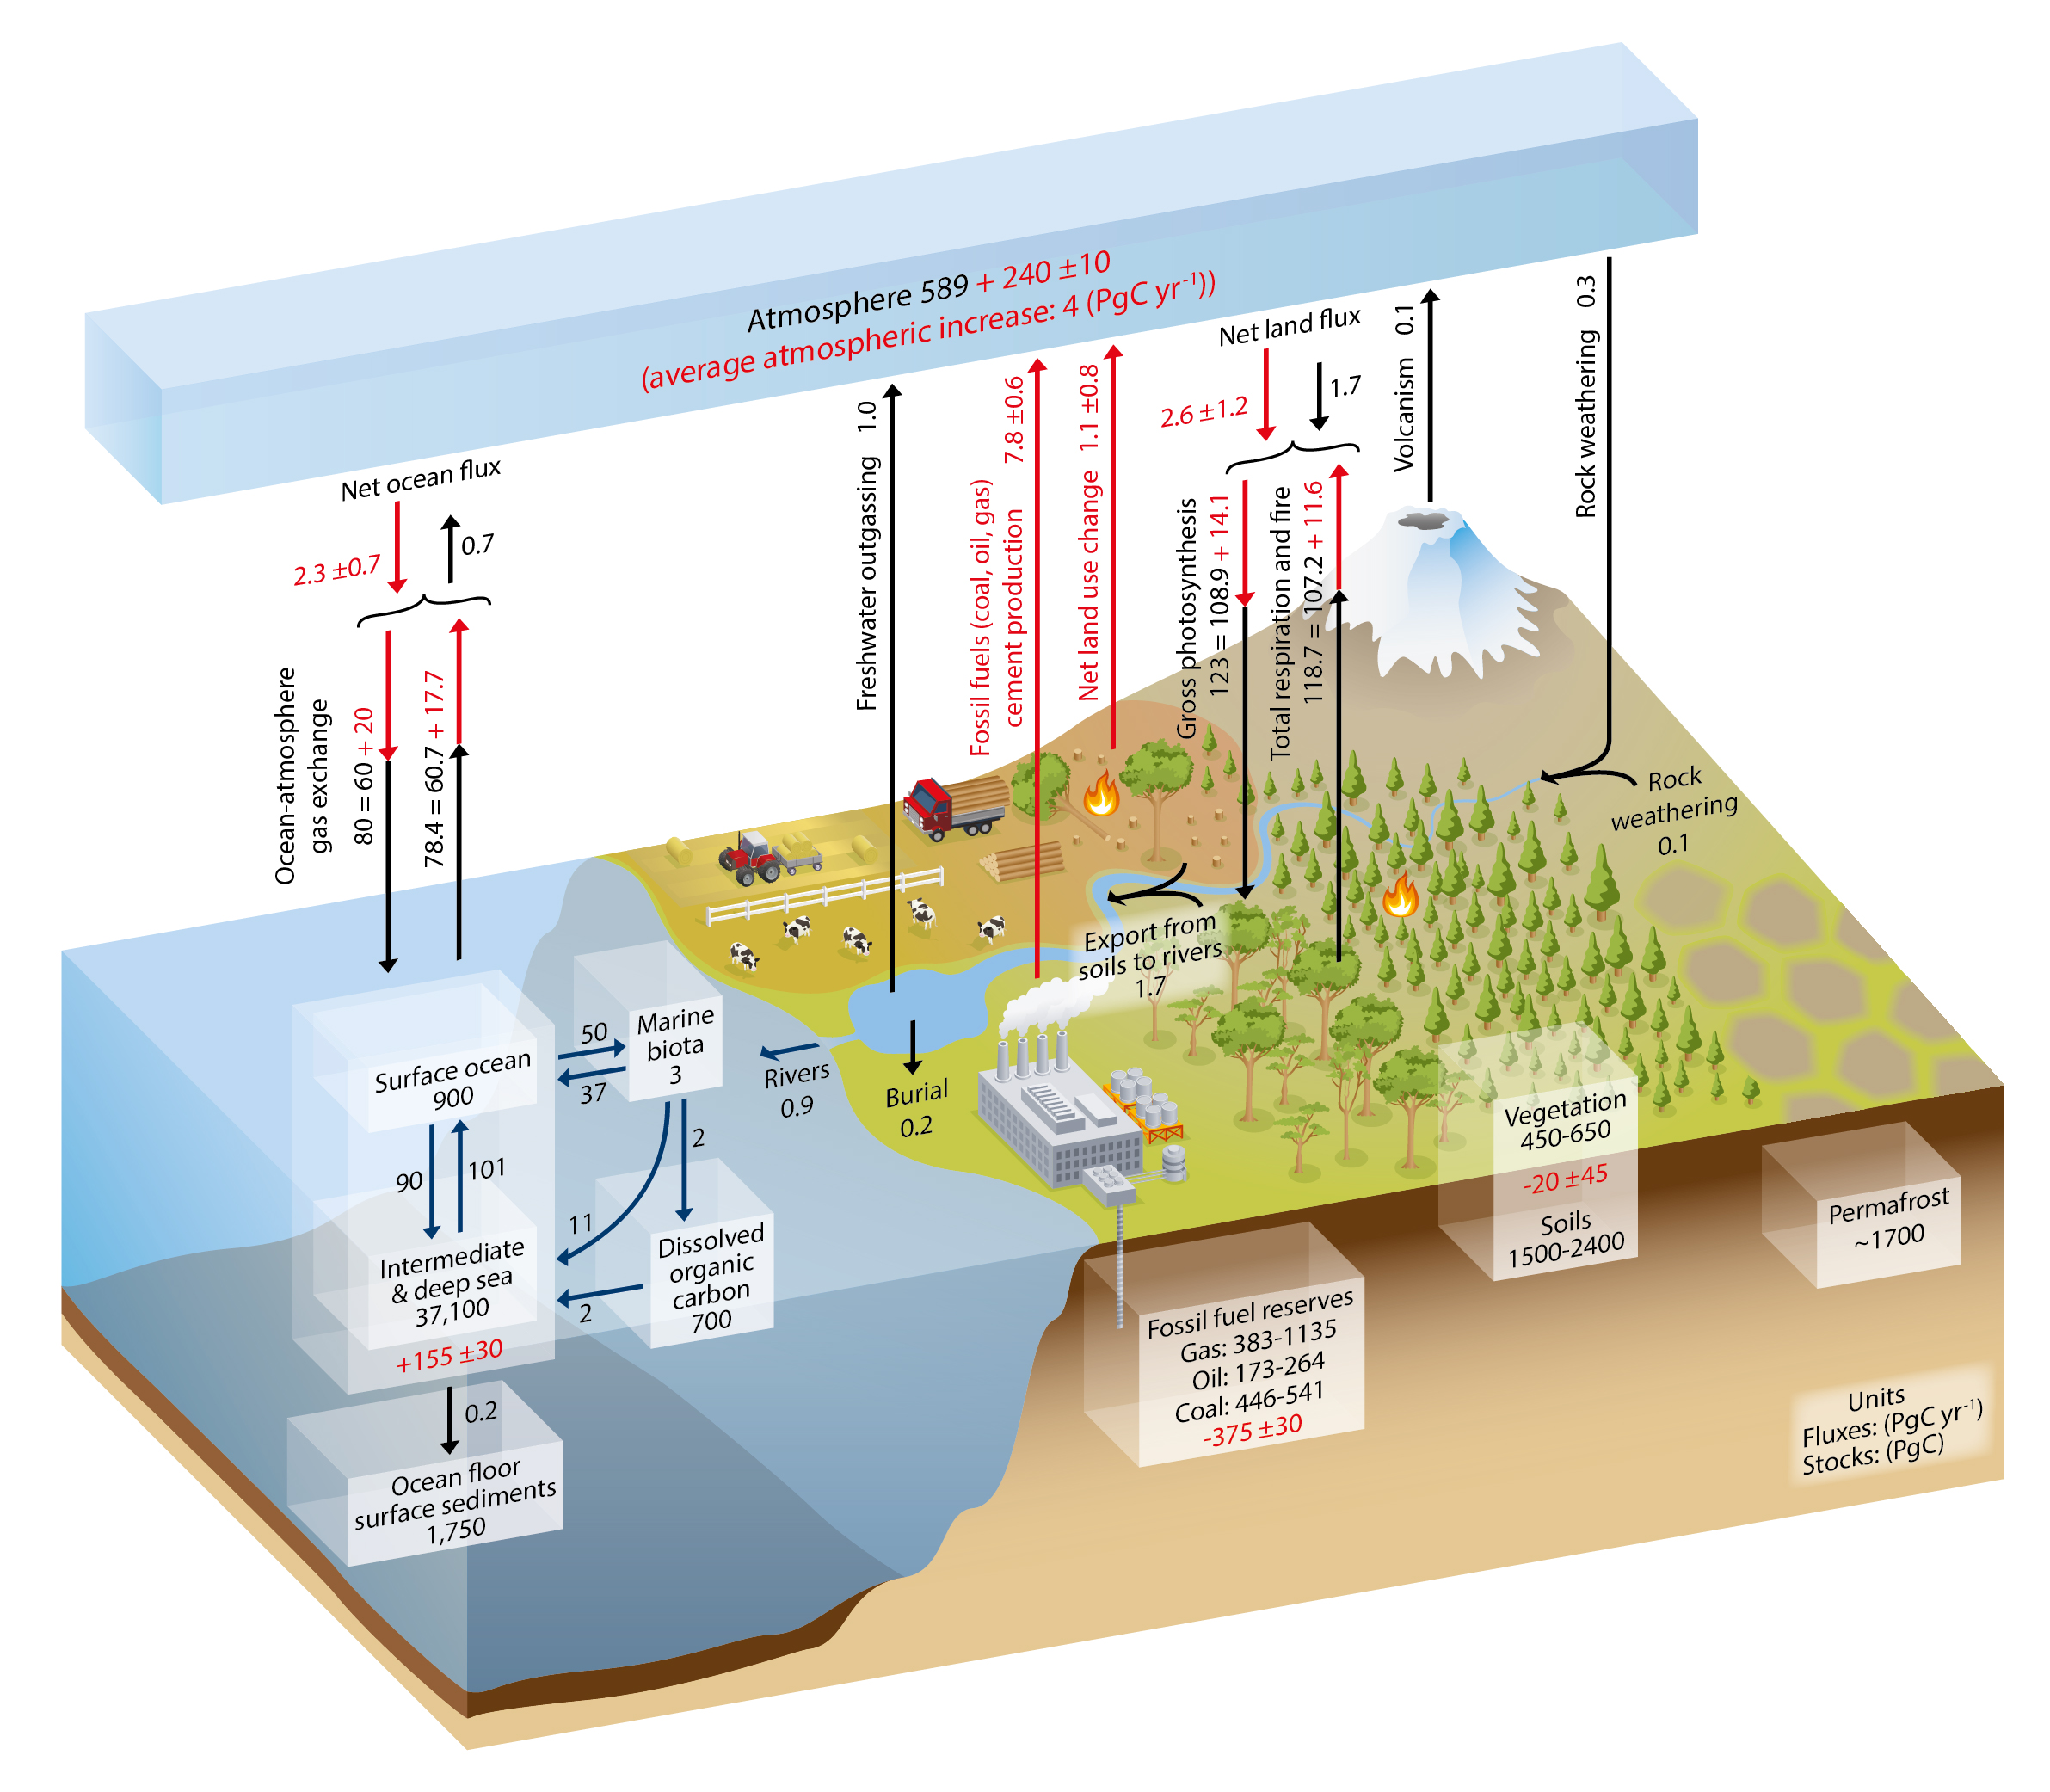
\includegraphics[width=0.9\textwidth]{chapter/chapter1/ipcc_fig6_1.jpg}
    \caption{Global carbon cycle simplified schematic \citep{ciais2014carbon}. Black numbers and arrows represent reservoir mass and exchange fluxes estimated for the time prior to the industrial era (\(\sim\)~1750). Red numbers and arrows represent annual fluxes averaged over the 2000-2009 time period. Red numbers in the reservoirs indicate the cumulative change of carbon over the industrial period (1750-2011).}
    \label{chap1:fig:ipcc_fig6.1}
\end{figure}

As atmospheric CO\(_{2}\) levels have risen, natural sinks of CO\(_{2}\) (fluxes out of the atmosphere) have intensified with both the land surface and oceans absorbing more CO\(_{2}\) from the atmosphere than in pre-industrial times. This can be see in figure~\ref{chap1:fig:ipcc_fig6.1}, with the the net ocean flux of CO\(_{2}\) to the atmosphere decreasing from an estimated +0.7~Pg~C~yr\(^{-1}\) to -2.3~Pg~C~yr\(^{-1}\), and the land surface flux of CO\(_{2}\) to the atmosphere decreasing from -1.7~Pg~C~yr\(^{-1}\) to -2.6~Pg~C~yr\(^{-1}\). More recent estimates from \citet{le2015global} indicate these sinks have further intensified with the ocean sink estimated to be 2.9 \(\pm 0.5\)~Pg~C~yr\(^{-1}\) and the land surface sink 4.1 \(\pm 0.9\)~Pg~C~yr\(^{-1}\) for the year 2014. The intensification of the land carbon sink is thought to be partly due to a combination of forest regrowth as well as rising CO\(_{2}\) and increased nitrogen deposition having a fertilisation effect \citep{ciais2014carbon}. It has also been shown that the land surface sink has been enhanced by an increase in diffuse photosynthetically active radiation as a result of increased cloud cover associated with increased anthropogenic emissions \citep{Mercadodiffuseradiation2009}. 

The partitioning of global carbon fluxes between emissions and sinks is important to better model the carbon cycle. However, current estimates are subject to high levels of uncertainty, which are reflected by the errors shown in Figure~\ref{chap1:fig:ipcc_fig6.1}. Current best estimates of global CO\(_{2}\) emissions and their partitioning between atmospheric growth rate and sinks are shown in Figure~\ref{chap1:fig:ipcc_fig6.8}. It is vitally important to understand the future response of sinks of CO\(_{2}\) (land surface and oceans) to climate change. If either the oceans or land surface were to stop absorbing the same percentage of CO\(_{2}\), we would see even more dramatic increases in atmospheric CO\(_{2}\) levels and thus a much greater rate of global warming. There is a high level of confidence that ocean carbon uptake will continue under all future emission scenarios \citep{ciais2014carbon}. There is much less confidence for the land surface and \citet{1748-9326-7-2-024002} have shown that global warming is particularly sensitive to land surface carbon cycle processes, highlighting the need to improve understanding of land surface carbon uptake. Some estimates show the land surface changing from a sink of CO\(_{2}\) to a source of CO\(_{2}\) under certain future emission scenarios \citep{sitch2008evaluation, cox2000, scholze2006climate}. In the latest IPCC report land surface carbon uptake is still considered the least understood process in the global carbon cycle \citep{ciais2014carbon}.

\begin{figure}[ht]
    \centering
    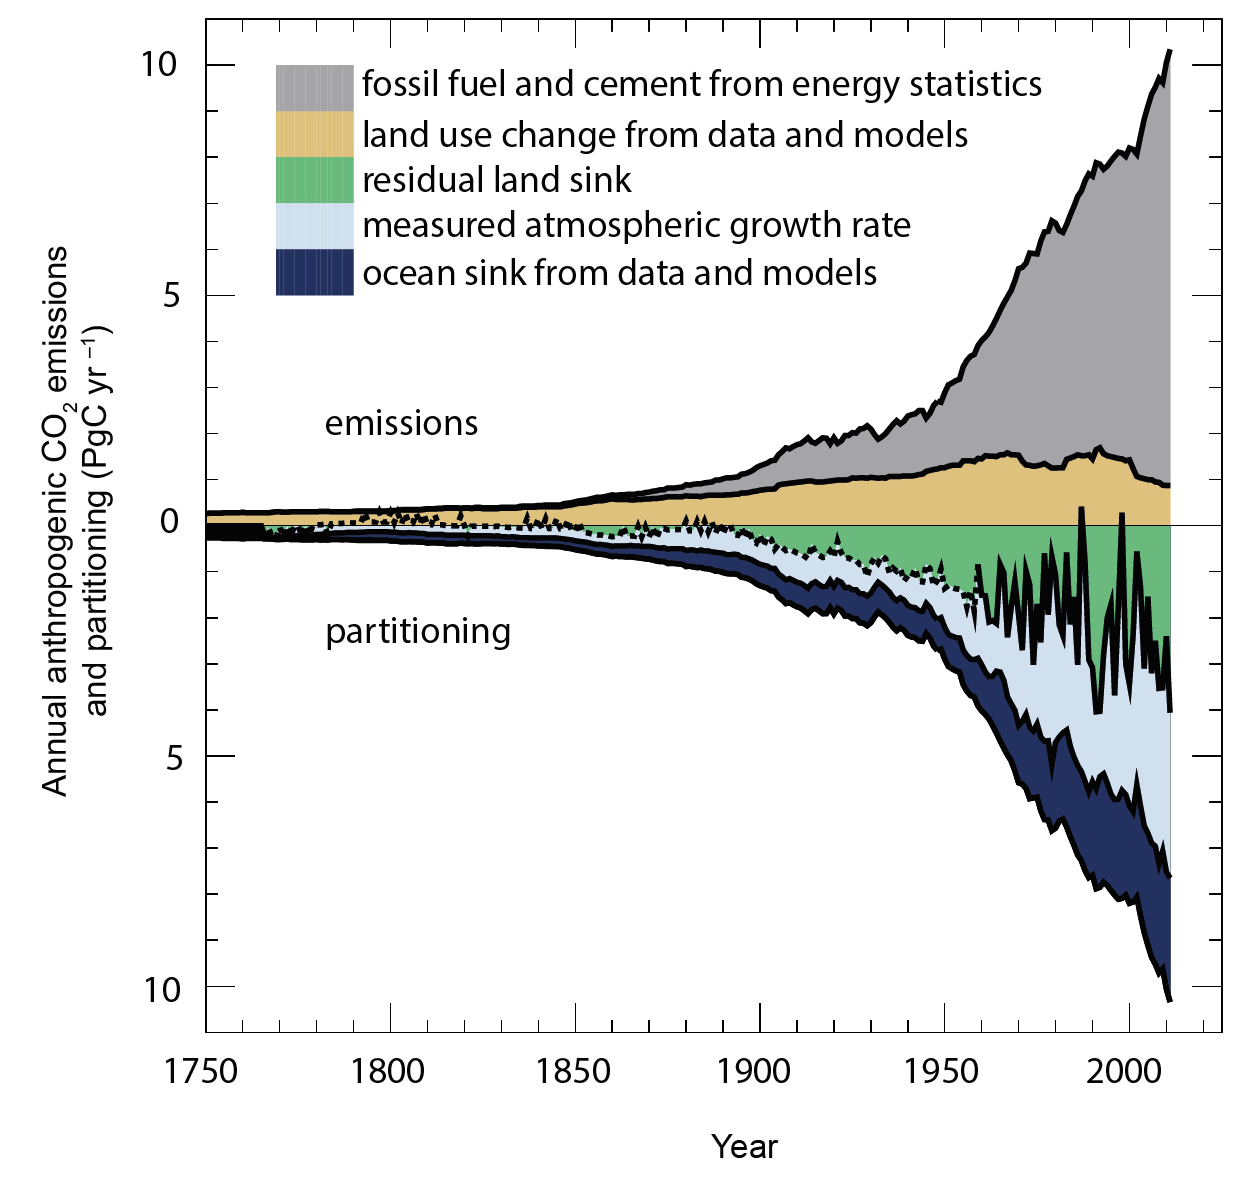
\includegraphics[width=0.9\textwidth]{chapter/chapter1/ipcc_fig6_8.jpg}
    \caption{Annual anthropogenic CO\(_{2}\) emissions and their partitioning among the atmosphere, land and ocean from 1750 to 2011  \citep{ciais2014carbon}.}
    \label{chap1:fig:ipcc_fig6.8}
\end{figure}

Currently land surface carbon uptake is estimated by taking the residual of all other calculated sources and sinks of carbon, so that
\begin{equation}
S_{LAND} = E_{FF} + E_{LUC} - (G_{ATM} + S_{OCEAN})
\end{equation}  
where \(S_{LAND}\) is the global residual land sink of CO\(_{2}\), \(E_{FF}\) is the CO\(_{2}\) emissions from fossil fuels, \(E_{LUC}\) is the CO\(_{2}\) emissions from land use change (mainly deforestation), \(G_{ATM}\) is the atmospheric CO\(_{2}\) growth rate and \(S_{OCEAN}\) is the mean ocean CO\(_{2}\) sink \citep{le2015global}. Figure~\ref{chap1:fig:ipcc_fig6.8} shows the growth in the estimated residual land sink as emissions increase. The high variability shown in this sink is largely due to the fact that it contains the residual errors of the four other terms. However, the land sink also displays some variability due to its sensitivity to year to year variations in precipitation, surface temperature, radiation and volcanic eruptions. Figure~\ref{chap1:fig:ipcc_fig6.8} shows that in 1986 and 1997 the land sink drops to zero, both of these years were among the strongest El Ni\~no's in recent history. In 1997 tropical droughts, often associated with El Ni\~no, were particularly severe leading to wildfires that released vast amounts of stored carbon \citep{schimel2013climate}.

%{\color{red} Include ecosystem flux description and figure here}
Terrestrial ecosystems are made up of autotrophs (organisms capable of photosynthesis) and heterotrophs (organisms that feed on organic carbon). The Gross Primary Productivity (GPP) of an ecosystem is the total amount of carbon removed from the atmosphere by photosynthesis. The Total Ecosystem Respiration (TER) is made up of autotrophic respiration (e.g. from plants) and heterotrophic respiration (e.g. from soil and litter organisms). The total carbon uptake or Net Ecosystem Exchange (NEE) of CO\(_2\) is then equal to -GPP+RT. A representation of these fluxes for a forest ecosystem are shown in Figure~\ref{chap1:fig:eco_fluxes}. 

\begin{figure}[ht]
    \centering
    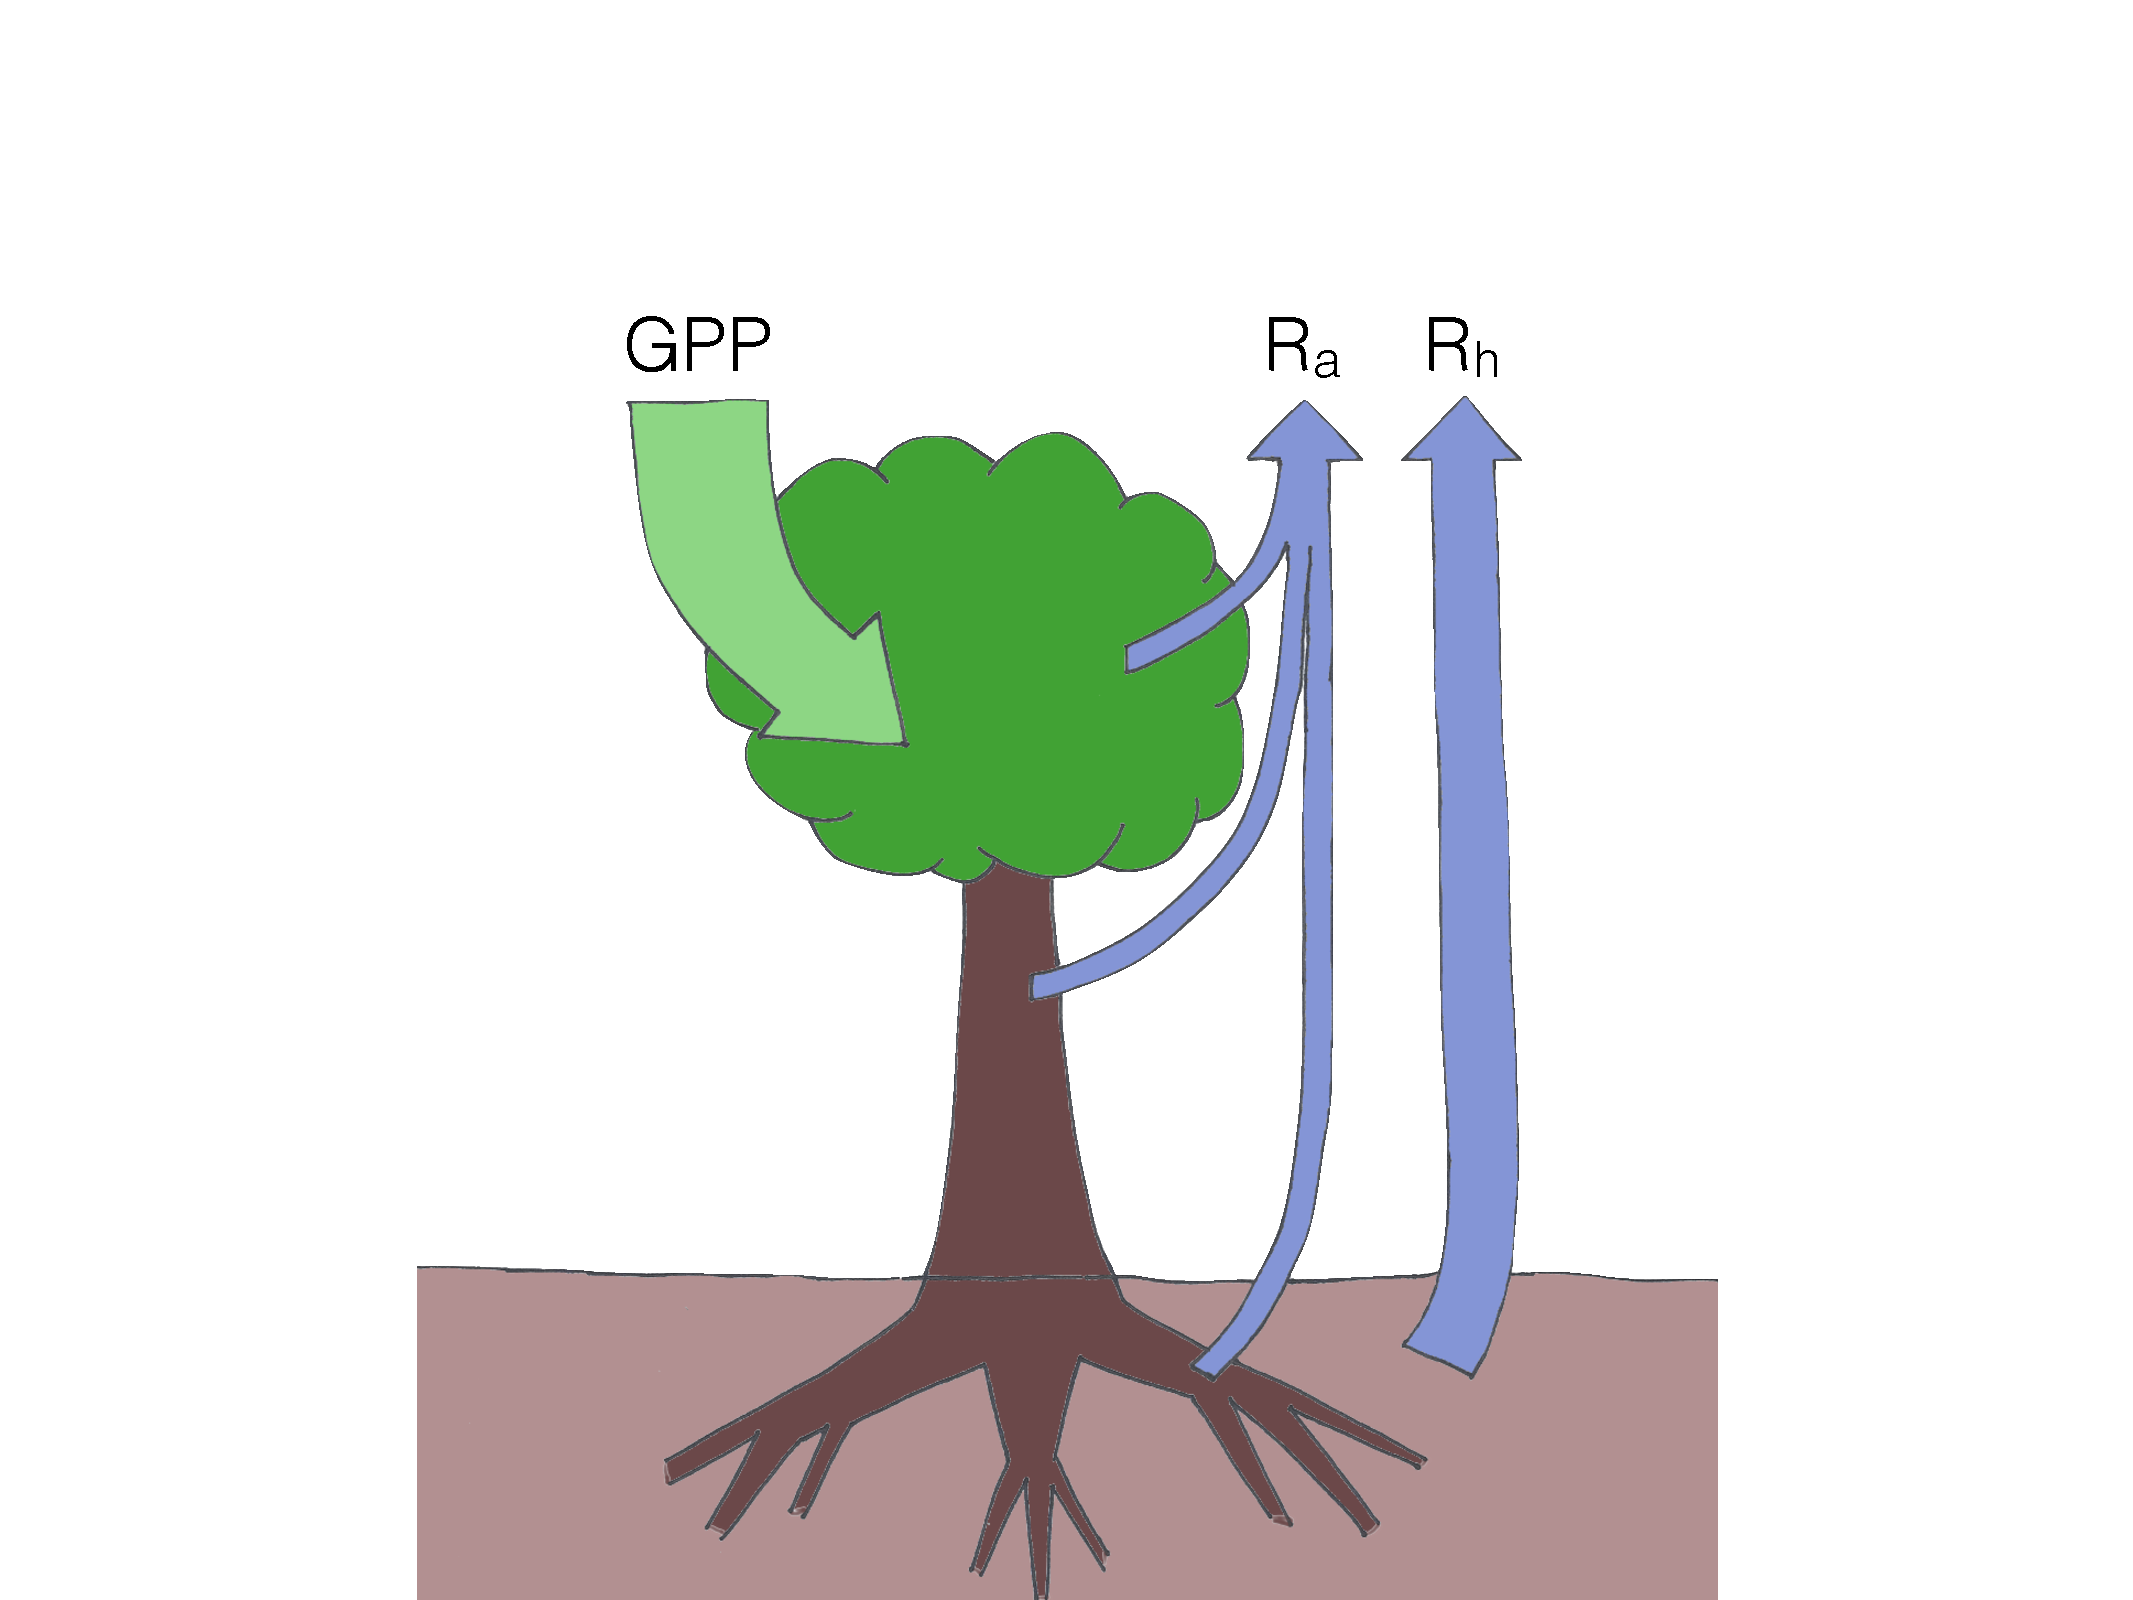
\includegraphics[width=0.5\textwidth]{chapter/chapter1/flux.pdf}
    \caption{Fluxes of carbon through a forest ecosystem. Gross Primary Productivity (GPP) represents total photosynthesis, R\(_{\text{a}}\) is autotrophic respiration from foliage, wood and roots, R\(_{\text{h}}\) is heterotrophic respiration from soil and litter. Total ecosystem respiration of carbon to the atmosphere (RT) is equal to R\(_{\text{a}}\) + R\(_{\text{h}}\). The Net Ecosystem Exchange (NEE) of CO\(_{2}\) is equal to -GPP + RT.}
    \label{chap1:fig:eco_fluxes}
\end{figure}

Disturbance of terrestrial ecosystems from fire, felling and insect outbreak can have significant impacts on carbon dynamics. Land use change is the second largest anthropogenic source of CO\(_{2}\). However, It is not well understood how much CO\(_{2}\) is removed from the atmosphere by regrowth of previously disturbed ecosystems (either by felling or fire), although it is thought that regrowth of forests in partcular could be stronger carbon sinks than their predecessors, due to more rapid biomass accumulation under succession \citep{pan2011large}. Better understanding the response of the land surface to disturbance will help constrain future carbon budgets. 

%Good paper to highlight the fact that the percentage of CO\(_{2}\) absorbed by the land surface has remained approximately constant with rising atmospheric CO\(_{2}\) levels??? Maybe just use IPCC fig 6.8?

%In figure 6.1 and 6.8: Partitioning of fluxes important and hard (shown by error on estimates in fig 6.1). Land surface carbon uptake least understood mechanism in the global carbon cycle, ref IPCC. Will uptake remain the same under climate change.

%Human emissions of CO\(_{2}\) have perturbed the global C cycle and caused a large continual increase in atmospheric CO\(_{2}\) levels.

%Look at papers recommended on Flux Course, some good ones to reference???

%IPCC figure 6.1 and 6.8: Partitioning of fluxes important and hard (shown by error on estimates in fig 6.1). Land surface carbon uptake least understood mechanism in the global carbon cycle, ref IPCC. Will uptake remain the same under climate change.

%\citet{1748-9326-7-2-024002} Have shown that global warming is highly sensitive to land carbon cycle processes and highlighted the need to improve understanding of land surface carbon uptake and its response to climate change. 

\section{Observations of terrestrial carbon balance}

There are an increasing number of available observations relevant to understanding the carbon balance of forests and the terrestrial biosphere. These observations include a range of variables, perhaps two of the most common are the Net Ecosystem Exchange (NEE) of CO\(_{2}\) and Leaf Area Index (LAI), which is the area of leaves per unit area ground. These variables can be directly measured at site level and can also be estimated from satellite remote sensing. Both NEE and LAI are important variables for understanding the carbon balance of ecosystems, with NEE giving us a direct estimate of the carbon uptake of an ecosystem and LAI being a main driver for the amount of GPP an ecosystem can perform.

%para on flux network and site level data:
At site level, flux towers measuring ecosystem-atmosphere fluxes of CO\(_{2}\), water and energy using the micrometeorological technique of eddy covariance provide one of the most valuable sources of information. Direct observations of ecosystem CO\(_{2}\) uptake are made at a fine temporal resolution, with observations every half-hour. A global flux network (FLUXNET), was established in 1997 \citep{baldocchi2001fluxnet}, to consolidate the information from a growing number of flux tower sites. Currently there are 517 active FLUXNET sites which are shown in Figure~\ref{chap1:fig:fluxnet_2015}, as can be seen these sites are not uniformly distributed so it is not possible to use FLUXNET sites alone to produce global estimates of terrestrial CO\(_{2}\) balance. However, these sites do provide an invaluable resource for model and satellite calibration. In turn this can be used to produce estimates on a global scale. At many flux tower sites and forest stands other diverse observations relevant to terrestrial carbon budgets are also being made. These include observations of soil and litter respiration, woody biomass and LAI. However, because they are labour intensive these observations are made much less frequently.     

\begin{figure}[ht]
\centering
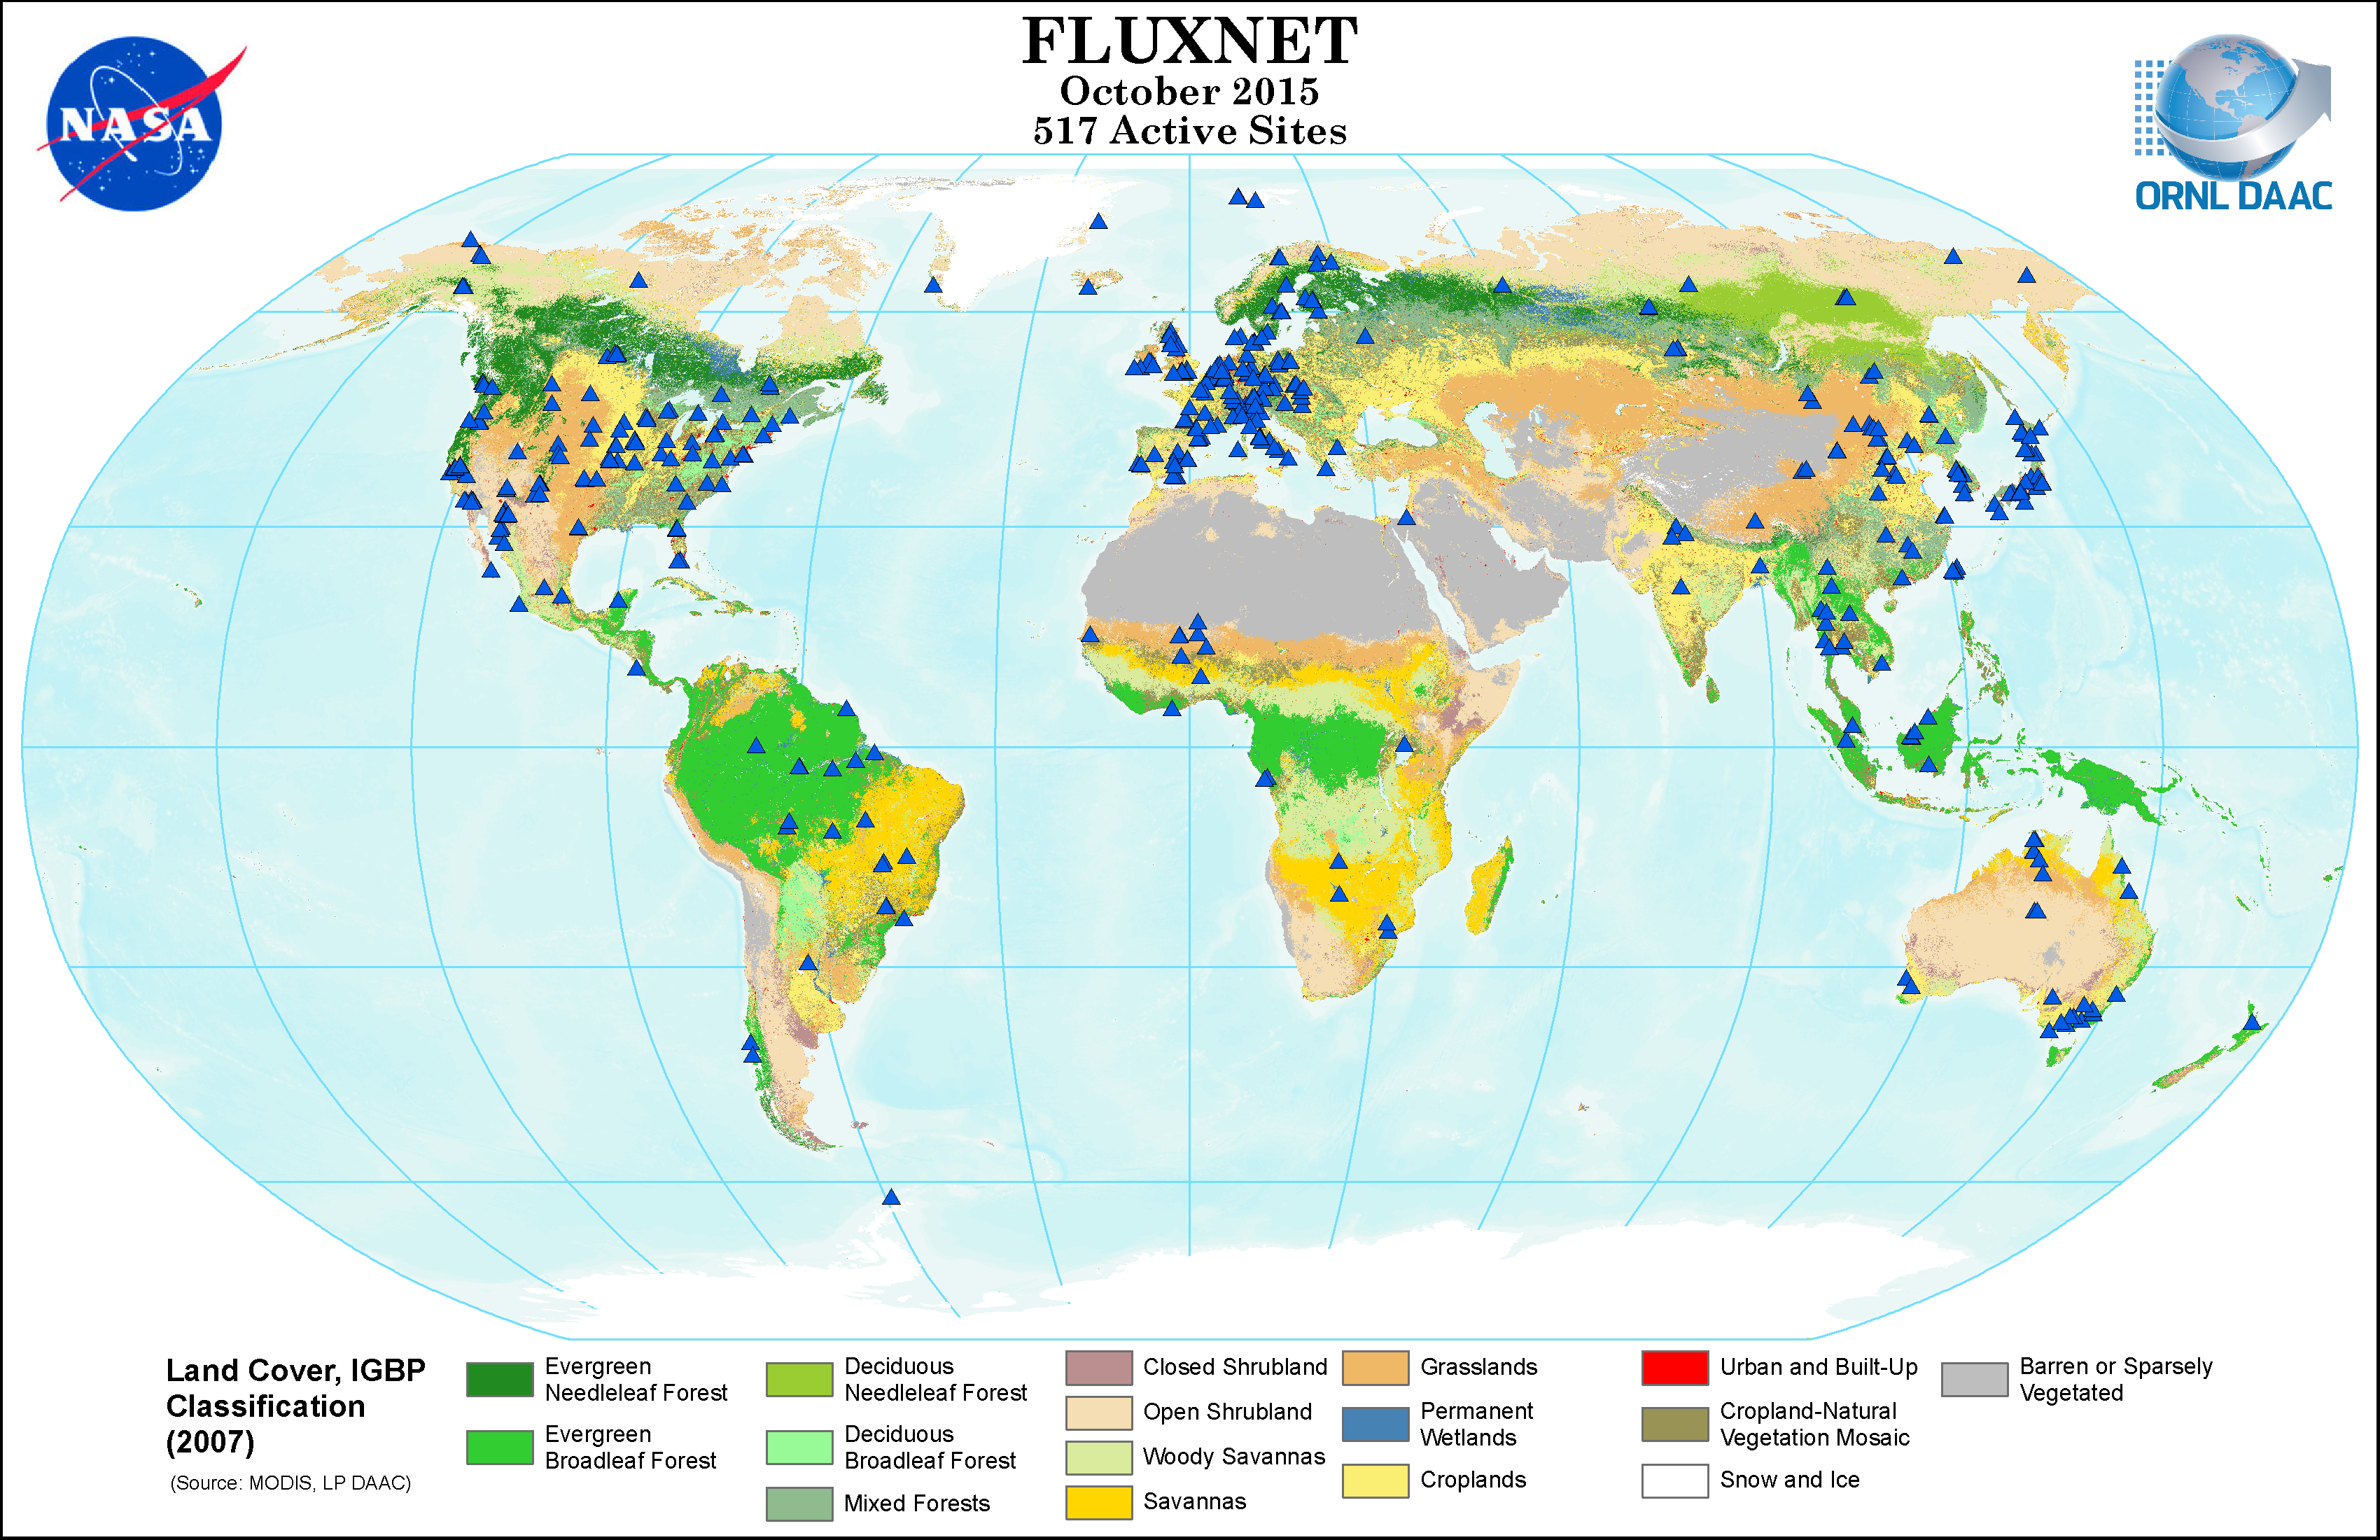
\includegraphics[width=0.9\textwidth]{chapter/chapter1/FluxNetworkMODIS_IGBP_10-2015.png}
\caption{FLUXNET sites and land cover (MODIS IGBP classification) \citep{fluxnetsite2013}.}
\label{chap1:fig:fluxnet_2015}
\end{figure}

%para on satellite data
The Moderate Resolution Imaging Spectroradiometer (MODIS) on the TERRA and AQUA satellites produces global estimates of LAI and Gross Primary Productivity (GPP) for terrestrial ecosystems \citep{running2004continuous}. However, MODIS actually measures reflected sunlight, this is then converted to vegetation indices, such as the Normalised Difference Vegetation Index (NDVI). These indices are correlated with the fraction of absorbed visible sunlight to estimate LAI or used in simple algorithms to estimate GPP \citep{yuan2007deriving}. It is therefore important to understand the limitations when interpreting satellite products as they do not represent direct observations. For LAI it has been shown that remotely sensed estimates saturate when measuring ecosystems with a LAI above 3 \citep{myneni2002global}. Terrestrial fluxes of carbon estimated from satellite measurements are subject to large errors in representativity, as satellites view a scene almost instantaneously and then derive daily mean fluxes \citep{baldocchi2008turner}. 
%Baldocchi paper: Many observations of forest carbon flux made worldwide.

\section{The role of models}

Observations can only tell us about the current and past state of a system. In order to produce future predictions and better understand current terrestrial carbon dynamics we must use mathematical models. Figure~\ref{chap1:fig:ipcc_fig6.16} show a comparison of the residual land sink (described in section~\ref{chap1:sec:global_c_cycle}) with the global terrestrial CO\(_{2}\) sink estimated from different process based global carbon cycle models. We see that although there is a high variability between modelled estimates there is good agreement between the multi-model mean and the residual land sink. 

\begin{figure}[ht]
    \centering
    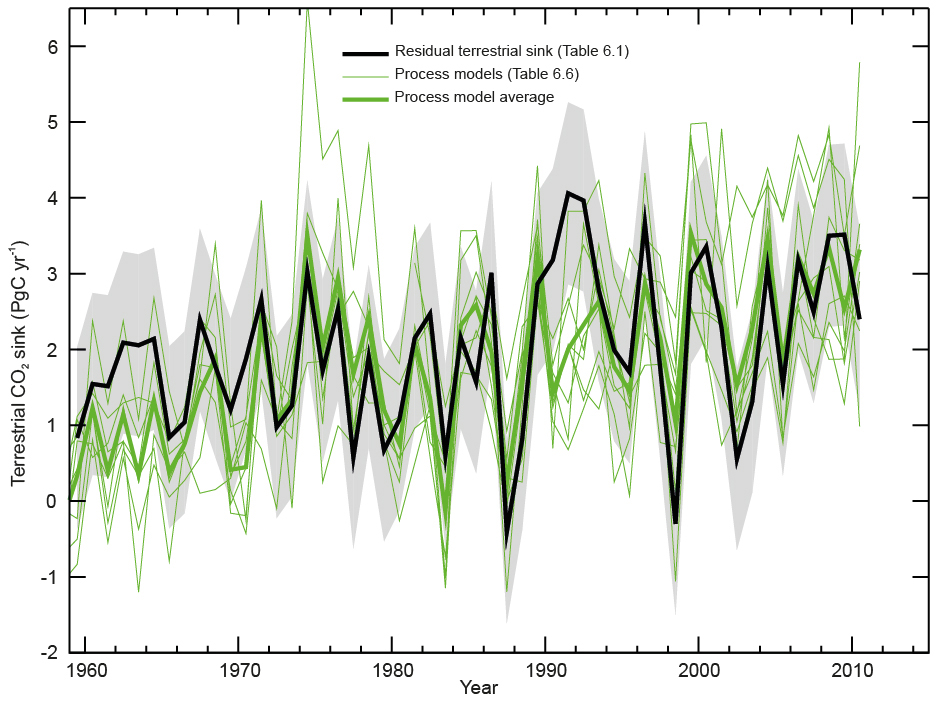
\includegraphics[width=0.9\textwidth]{chapter/chapter1/ipcc_fig6_16.jpg}
    \caption{Comparison of the residual land sink (black line) with the global terrestrial CO\(_{2}\) sink estimated from different process based global carbon cycle models \citep{ciais2014carbon}. Grey shading represents uncertainty in residual land sink.}
    \label{chap1:fig:ipcc_fig6.16}
\end{figure}

Representative Concentration Pathways (RCPs) of CO\(_{2}\) concentrations and emissions have been developed \citep{moss2010next} to drive climate models to produce future predictions. Under these pathways land surface carbon uptake is highly uncertain with little agreement between different process based models. Some predict the land surface to become a source of CO\(_{2}\) and others predict a further intensification of the residual land sink \citep{jones2013twenty}. This large uncertainty for land surface models is partly due to poor model parameterisations and missing processes within models. One of the main processes many current global models do not account for is the effect of disturbance on terrestrial ecosystem carbon dynamics.

It has been shown that many terrestrial carbon cycle models simulating the seasonal cycle of land-atmosphere CO\(_{2}\) exchange perform poorly when compared to FLUXNET sites in North America \citep{schwalm2010model}. Here a difference between observations and model predictions of 10 times the observational uncertainty was found, highlighting the need for continued model development. In order to improve global models of terrestrial carbon balance it is important to use site-level-research to hone the processes and parameterisations of the models where we have diverse sets of direct observations with which to judge modified-model performance. 
%IPCC figure 6.16 and section 6.3.2.6.6: Contribution of models to understanding the terrestrial carbon cycle. Reference every DALEC paper.


\section{Data assimilation}

%{\color{red} Observations are sparse, current model predictions are poor, data assimilation provides a way to combine both sources of information to improve current estimates.}

As discussed above, the level of uncertainty in terrestrial carbon balance predictions arise from significant gaps in the direct observations available and from a lack of clarity and authoritative parameterisation of the constituent processes in current models. The technique of data assimilation provides a method for combining and comparing the output of predictive models with incomplete observations to find the best estimate for the state and parameters of a system. Data assimilation has had many successful applications. Perhaps the most important application has been in numerical weather prediction where data assimilation has contributed to forecast accuracy being increased at longer lead times, with the result that the four day forecast in 2014 now has the same level of accuracy as the one day forecast in 1979 \citep{bauer2015quiet}. Obviously, this improved forecasting is not solely due to data assimilation but also increased quality and resolution of observations along with improvements in model structure, however the introduction and evolution of data assimilation has been a key part of the improvement \citep{dee2011era}.

More recently data assimilation has been used to improve our knowledge of ecological systems. For the carbon balance of forests it has been used to combine many different observations with functional ecology models \citep{zobitz2011primer, fox2009reflex, richardson2010estimating, Quaife2008, Zobitz2014, Niu2014}. Global land surface models have also been implemented with data assimilation, mainly using data from satellite and atmospheric $\text{CO}_{2}$ observations \citep{Kaminski2013, scholze2007propagating}. In a few cases site level data has also been assimilated \citep{Verbeeck2011, Bacour2015}. In comparison with numerical weather prediction, the use of data assimilation in these areas is relatively new and underdeveloped. The further application of data assimilation to models of ecosystem carbon balance will help to improve model parameterisations and future predictions. The development of improved data assimilation techniques will also help to  identify missing model processes and changes in model parameters and behaviour over time. In particular, understanding the change in model parameters over time will be of use in improving models predictions of the effect of disturbance in terrestrial ecosystems.
  
%Role of DA in NWP improving forecast skill. 


%
%\include{eng_review}
%
%\include{lin_elast_finite_elements}
%
%\include{opt_review}
%
%\include{min_comp_st_vol}
%
%\include{buckling}
%
%\include{analysis_eso}
%
%%Chapter 1

This thesis has explored data assimilation for the terrestrial carbon cycle. The state of the global carbon cycle in the IPCC AR5 suggests that the land surface is the most uncertain component of the global carbon cycle. The response of ecosystem carbon uptake to land use change and disturbance (e.g. fire, felling, insect outbreak) is a large component of this uncertainty. The uncertainties in land surface carbon cycling processes are largely due to gaps in direct observations and poor parameterisations of model processes. Data assimilation provides methods to improve current estimates by combining observations with prior model estimates. In order to improve data assimilation results it is important that we add the most possible information about a system to data assimilation schemes. The equates to large amounts and more accurate information in, equals better information out. This could mean new observations with high levels of information for constraining poorly understood processes, or better characterisation of prior model and observational errors. Both the optimal set of observations and appropriate representation of error in data assimilation for the carbon cycle are not well understood. Based on this and knowledge of other components of uncertainty three key areas of research were identified in chapter~\ref{chap:intro}:
\begin{enumerate}
\item \textit{Investigating the information content in distinct carbon balance observations for data assimilation}

\item \textit{Improving the representation of prior and observational errors in carbon cycle data assimilation}

\item \textit{Using data assimilation to understand the effect of disturbance on forest carbon dynamics}
\end{enumerate}
The following sections will address these points in turn based on the work presented in this thesis in chapter~\ref{chap:info_con}--\ref{chap:disturbance}.

\section{Investigating the information content in distinct carbon balance observations for data assimilation}

In chapter~\ref{chap:info_con} we used both the DALEC1 and DALEC2 models of ecosystem carbon balance in a series of information content experiments. We calculated the tangent linear model of DALEC1 analytically by hand so that we could make novel applications of information content metrics relying on the adjoint of the model code. For the more complex and nonlinear DALEC2 joint state and parameter estimation case the tangent linear model was calculated using automatic differentiation. From the information content experiments in this chapter we deduced the following conclusions:
\begin{itemize}
\item For both the DALEC1 and DALEC2 models we found our system was observable for the available observations of NEE. This means that for data assimilation we can construct a locally unique solution from observational information alone. This is important as it give us confidence in subsequent experimental results relying on NEE as the main source for observational information.
\item There was a strong temporal variation in information content for observations of NEE, with observations made at times of higher temperatures having higher information content. For deciduous ecosystems observations of NEE made at times of leaf-on and leaf-off have higher influence in the assimilation as these act to help constrain the phenology of the model. 
\item Including an increasing correlation between NEE observation errors in time reduced the information content in the assimilated observations. 
\item It was clear from these experiments that in order to further improve understanding of the information content in observations it is important to improve estimates and representations of uncertainty for both prior model predictions and observations.
\end{itemize}

\section{Improving the representation of prior and observational errors in carbon cycle data assimilation}

In chapter~\ref{chap:error_corrs} we implemented and tested a 4D-Var data assimilation scheme with the DALEC2 model. We then used this system to investigate the effect of including correlations between prior model and NEE observation errors. In each experiment we assimilated a single year of NEE observations (1999) and then ran a 14 year forecast (2000-2014) of NEE. From this work our conclusions were:
\begin{itemize}
\item Including correlations in the background error covariance matrix significantly improved the model forecast after assimilation. Correlations in the observation error covariance matrix between NEE observation errors in time had much less of an effect on results. However, we expect these correlations will have more impact when assimilating more than one data stream or assimilating observations of NEE at a finer temporal resolution.
\item When correlations were included in both the background error covariance matrix and the observation error covariance matrix we found the best model forecast results. In this case the forecast root-mean-square error was reduced by a significant $44\% $ in comparison to when a diagonal background and observation error covariance matrix were used in assimilation.
\end{itemize} 


\section{Using data assimilation to understand the effect of disturbance on forest carbon dynamics}

In chapter~\ref{chap:disturbance} we again utilised the 4D-Var data assimilation scheme with DALEC2 outlined in chapter~\ref{chap:error_corrs} along with a set of observations taken on a fieldwork campaign to investigate the effect of selective felling on the carbon dynamics of the Alice Holt forest. We conducted a data-denial experiments using all the available observations to understand their effect on the modelled predicted effect of disturbance. We also propose novel observation operators allowing for the assimilation of daytime and nighttime NEE observations with a daily time-step model. The main results in this chapter were as follows:
\begin{itemize}
\item The proposed observation operators allow our model to accurately predict daytime and nighttime NEE and negate the need for any model modification. 
\item We find no change to the net ecosystem carbon uptake after felling when approximately 46\% of trees were removed from the area of interest.
\item Our most confident modelled estimate (when all available data is assimilated) suggests this unchanged carbon uptake is due to GPP being the main driver for both autotrophic and heterotrophic respiration, so that even with reduced GPP post-disturbance the same NEE can occur due to significant reductions in total ecosystem respiration. We find different conclusions if we base our conclusions solely on the assimilation of NEE observations, highlighting the need for caution not to over-interpret results when assimilating only this variable. 
\end{itemize}

\section{Future work}

The continued application of information content measures is important to better understand where to base efforts in future observation campaigns. It is also important to improve estimates of uncertainty for both prior model predictions and observations. This will ensure that results from information content experiments can be as accurate as possible. It would also be interesting to use a more complex model of ecosystem carbon dynamics where we could judge the impact of more novel measurements such as stem respiration.

We have shown that including a more sophisticated representation of error in data assimilation schemes can be of great benefit to results. more work in this area is important to improve the representation of uncertainty in data assimilation schemes. In relation to the experiments carried out in this thesis its is clear that a more diagnostic tool for the specification of observation error correlations is important. One possibility for this would be to use a method such as the \citet{desroziers2005diagnosis} diagnostic to statistically estimate the error covariance structure of assimilated observations. In order to diagnose correlations in time (similar to those specified in chapter~\ref{chap:error_corrs}) the \citet{desroziers2005diagnosis} diagnostic would have to be expanded. The \citet{desroziers2005diagnosis} diagnostic estimates the observation error covariance matrix as
\begin{equation}
\textbf{R} = \mathbb{E}[(\textbf{y}-\textbf{h}(\textbf{x}_a))(\textbf{y}-\textbf{h}(\textbf{x}_b))^{T}]
\end{equation}
this could be re-written as
\begin{equation}
\hat{\textbf{R}} = \mathbb{E}[(\hat{\textbf{y}}-\hat{\textbf{h}}(\textbf{x}_a))(\hat{\textbf{y}}-\hat{\textbf{h}}(\textbf{x}_b))^{T}]
\end{equation}
to estimate time correlations in the observation error covariance matrix. This would require that an ensemble of 4D-Var data assimilations were run with perturbed prior model estimates and perturbed observations. We could then retrieve a statistical estimate of the temporal correlation structure for the observation error covariance matrix. It will also be useful to test these new covariance matrices with included correlations at other research sites and with larger model implementations.

The results we find for the effect of disturbance are possibly surprising however do support ecological measurement campaigns analysing soil microbial communities after selective felling events. This experiment would be good to carry out again after collecting a few more years of data to understand the recovery of leaf area and long term response of the Alice Holt forest to disturbance. If possible it would be extremely beneficial to also set up soil respiration chambers on both the thinned and unthinned sides of the forest to improve constraint on the constituent processes.
%\clearpage
%\thispagestyle{empty}
%\hspace{1cm}
%\clearpage

\appendix

\begin{table}[h!]
  %  \footnotesize
  \caption{\label{tab:models_full}The CMIP5 multi-model ensemble official groups, names and ensemble numbers.}
  \centering
  %\vspace{6pt}
  \begin{tabular}{m{6cm}m{5cm}cc} \hline
    \textbf{Modeling Center (or Group)} & \textbf{Model} & \textbf{Experiment} & \textbf{Ensemble} \\ \hline \hline
    \multirow{8}{\linewidth}{Commonwealth Scientific and Industrial Research Organization (CSIRO) and Bureau of Meteorology (BOM), Australia} & \multirow{4}{\linewidth}{ACCESS1.0\\ \citep{Collier2012}} & AMIP & r1i1p1 \\ \cline{3-4}
     &  & Historical & r1i1p1 \\ \cline{3-4}
     &  & RCP4.5 & r1i1p1 \\ \cline{3-4}
     &  & RCP8.5 & r1i1p1 \\ \cline{2-4}
     & \multirow{4}{\linewidth}{ACCESS1.3\\ \citep{Collier2012}} & AMIP & r1i1p1 \\ \cline{3-4}
     &  & Historical & r1i1p1 \\ \cline{3-4}
     &  & RCP4.5 & r1i1p1 \\ \cline{3-4}
     &  & RCP8.5 & r1i1p1 \\ \hline
    \multirow{16}{\linewidth}{Beijing Climate Center, China Meteorological Administration} & \multirow{8}{\linewidth}{BCC-CSM1.1\\ \citep{Xin2013}} & \multirow{3}{*}{AMIP} & r1i1p1 \\
     &  &  & r2i1p1 \\
     &  &  & r3i1p1 \\ \cline{3-4}
     &  & \multirow{3}{*}{Historical} & r1i1p1 \\
     &  &  & r2i1p1 \\
     &  &  & r3i1p1 \\ \cline{3-4}
     &  & RCP4.5 & r1i1p1 \\ \cline{3-4}
     &  & RCP8.5 & r1i1p1 \\ \cline{2-4}
     & \multirow{8}{\linewidth}{BCC-CSM1.1(m)\\ \citep{Xin2013}} & \multirow{3}{*}{AMIP} & r1i1p1 \\
     &  &  & r2i1p1 \\
     &  &  & r3i1p1 \\ \cline{3-4}
     &  & \multirow{3}{*}{Historical} & r1i1p1 \\
     &  &  & r2i1p1 \\
     &  &  & r3i1p1 \\ \cline{3-4}
     &  & RCP4.5 & r1i1p1 \\ \cline{3-4}
     &  & RCP8.5 & r1i1p1 \\ \hline
    \multirow{4}{\linewidth}{College of Global Change and Earth System Science, Beijing Normal University} & \multirow{4}{\linewidth}{BNU-ESM\\ (Atmospheric component: CAM3.5 -- \citealt{Neale2008})} & AMIP & r1i1p1 \\ \cline{3-4}
     &  & Historical & r1i1p1 \\ \cline{3-4}
     &  & RCP4.5 & r1i1p1 \\ \cline{3-4}
     &  & RCP8.5 & r1i1p1 \\ \hline
    \hline \multicolumn{4}{r}{\textit{Continued on next page}} \\ \hline
  \end{tabular}
\end{table}
\begin{table}
  \centering
  \begin{tabular}{m{6cm}m{5cm}cc} \hline
    \multicolumn{4}{c}%
    {\tablename\ \thetable\ -- \textit{Continued from previous page}} \\
    \hline \textbf{Modeling Center (or Group)} & \textbf{Model} & \textbf{Experiment} & \textbf{Ensemble} \\ \hline \hline
    \multirow{7}{\linewidth}{Canadian Centre for Climate Modelling and Analysis} & \multirow{7}{\linewidth}{CanESM2\\ (Atmospheric component: AGCM4 -- based on \citealt{Scinocca2008})} & \multirow{5}{*}{Historical} & r1i1p1 \\
     &  &  & r2i1p1 \\
     &  &  & r3i1p1 \\
     &  &  & r4i1p1 \\
     &  &  & r5i1p1 \\ \cline{3-4}
     &  & RCP4.5 & r1i1p1 \\ \cline{3-4}
     &  & RCP8.5 & r1i1p1 \\ \hline
    \multirow{7}{\linewidth}{National Center for Atmospheric Research} & \multirow{7}{\linewidth}{CCSM4\\ \citep{Gent2011}} & \multirow{4}{*}{AMIP} & r1i1p1 \\
     &  &  & r2i1p1 \\
     &  &  & r3i1p1 \\
     &  &  & r4i1p1 \\ \cline{3-4}
     &  & Historical & r6i1p1 \\ \cline{3-4}
     &  & RCP4.5 & r6i1p1 \\ \cline{3-4}
     &  & RCP8.5 & r6i1p1 \\ \hline
    \multirow{6}{\linewidth}{Centro Euro-Mediterraneo per i Cambiamenti Climatici} & \multirow{6}{\linewidth}{CMCC-CM\\ \citep{Bellucci2012}} & \multirow{3}{*}{AMIP} & r1i1p1 \\
     &  &  & r2i1p1 \\
     &  &  & r3i1p1 \\ \cline{3-4}
     &  & Historical & r1i1p1 \\ \cline{3-4}
     &  & RCP4.5 & r1i1p1 \\ \cline{3-4}
     &  & RCP8.5 & r1i1p1 \\ \hline
    \multirow{13}{\linewidth}{Centre National de Recherches M\'{e}t\'{e}orologiques / Centre Europ\'{e}en de Recherche et Formation Avanc\'{e}es en Calcul Scientifique} & \multirow{13}{\linewidth}{CNRM-CM5\\ \citep{Voldoire2012}} & AMIP & r1i1p1 \\ \cline{3-4}
     &  & \multirow{10}{*}{Historical} & r1i1p1 \\
     &  &  & r2i1p1 \\
     &  &  & r3i1p1 \\
     &  &  & r4i1p1 \\
     &  &  & r5i1p1 \\
     &  &  & r6i1p1 \\
     &  &  & r7i1p1 \\
     &  &  & r8i1p1 \\
     &  &  & r9i1p1 \\
     &  &  & r10i1p1 \\ \cline{3-4}
     &  & RCP4.5 & r1i1p1 \\ \cline{3-4}
     &  & RCP8.5 & r1i1p1 \\ \hline
    \hline \multicolumn{4}{r}{\textit{Continued on next page}} \\ \hline
  \end{tabular}
\end{table}
\begin{table}
  \centering
  \begin{tabular}{m{6cm}m{5cm}cc} \hline
    \multicolumn{4}{c}%
    {\tablename\ \thetable\ -- \textit{Continued from previous page}} \\
    \hline \textbf{Modeling Center (or Group)} & \textbf{Model} & \textbf{Experiment} & \textbf{Ensemble} \\ \hline \hline
    \multirow{40}{\linewidth}{Commonwealth Scientific and Industrial Research Organization in collaboration with Queensland Climate Change Centre of Excellence} & \multirow{40}{\linewidth}{CSIRO-Mk3.6.0\\ \citep{Rotstayn2012}} & \multirow{10}{*}{AMIP} & r1i1p1 \\
     &  &  & r2i1p1 \\
     &  &  & r3i1p1 \\
     &  &  & r4i1p1 \\
     &  &  & r5i1p1 \\
     &  &  & r6i1p1 \\
     &  &  & r7i1p1 \\
     &  &  & r8i1p1 \\
     &  &  & r9i1p1 \\
     &  &  & r10i1p1 \\ \cline{3-4}
     &  & \multirow{10}{*}{Historical} & r1i1p1 \\
     &  &  & r2i1p1 \\
     &  &  & r3i1p1 \\
     &  &  & r4i1p1 \\
     &  &  & r5i1p1 \\
     &  &  & r6i1p1 \\
     &  &  & r7i1p1 \\
     &  &  & r8i1p1 \\
     &  &  & r9i1p1 \\
     &  &  & r10i1p1 \\ \cline{3-4}
     &  & \multirow{10}{*}{RCP4.5} & r1i1p1 \\
     &  &  & r2i1p1 \\
     &  &  & r3i1p1 \\
     &  &  & r4i1p1 \\
     &  &  & r5i1p1 \\
     &  &  & r6i1p1 \\
     &  &  & r7i1p1 \\
     &  &  & r8i1p1 \\
     &  &  & r9i1p1 \\
     &  &  & r10i1p1 \\ \cline{3-4}
     &  & \multirow{10}{*}{RCP8.5} & r1i1p1 \\
     &  &  & r2i1p1 \\
     &  &  & r3i1p1 \\
     &  &  & r4i1p1 \\
     &  &  & r5i1p1 \\
     &  &  & r6i1p1 \\
     &  &  & r7i1p1 \\
     &  &  & r8i1p1 \\
     &  &  & r9i1p1 \\
     &  &  & r10i1p1 \\ \hline
    \multirow{7}{\linewidth}{EC-EARTH Consortium} & \multirow{7}{\linewidth}{EC-EARTH\\\citep{Sterl2011}} & AMIP & r1i1p1 \\ \cline{3-4}
     &  & Historical & r9i1p1 \\ \cline{3-4}
     &  & \multirow{2}{*}{RCP4.5} & r8i1p1 \\
     &  &  & r12i1p1 \\ \cline{3-4}
     &  & \multirow{3}{*}{RCP8.5} & r6i1p1 \\
     &  &  & r8i1p1 \\
     &  &  & r12i1p1 \\ \hline
    \hline \multicolumn{4}{r}{\textit{Continued on next page}} \\ \hline
  \end{tabular}
\end{table}
\begin{table}
  \centering
  \begin{tabular}{m{6cm}m{5cm}cc} \hline
    \multicolumn{4}{c}%
    {\tablename\ \thetable\ -- \textit{Continued from previous page}} \\
    \hline \textbf{Modeling Center (or Group)} & \textbf{Model} & \textbf{Experiment} & \textbf{Ensemble} \\ \hline \hline
    \multirow{4}{\linewidth}{LASG, Institute of Atmospheric Physics, Chinese Academy of Sciences and CESS, Tsinghua University} & \multirow{4}{\linewidth}{FGOALS-g2\\ \citep{Wang2013}} & AMIP & r1i1p1 \\ \cline{3-4}
     &  & Historical & r3i1p1 \\ \cline{3-4}
     &  & RCP4.5 & r1i1p1 \\ \cline{3-4}
     &  & RCP8.5 & r1i1p1 \\ \hline
    \multirow{13}{\linewidth}{LASG, Institute of Atmospheric Physics, Chinese Academy of Sciences} & \multirow{12}{\linewidth}{FGOALS-s2\\ \citep{Bao2013}} & \multirow{3}{*}{AMIP} & r1i1p1 \\
     &  &  & r2i1p1 \\
     &  &  & r3i1p1 \\ \cline{3-4}
     &  & \multirow{3}{*}{Historical} & r1i1p1 \\
     &  &  & r2i1p1 \\
     &  &  & r3i1p1 \\ \cline{3-4}
     &  & \multirow{3}{*}{RCP4.5} & r1i1p1 \\
     &  &  & r2i1p1 \\
     &  &  & r3i1p1 \\ \cline{3-4}
     &  & \multirow{3}{*}{RCP8.5} & r1i1p1 \\
     &  &  & r2i1p1 \\
     &  &  & r3i1p1 \\ \hline
    \multirow{15}{\linewidth}{NOAA Geophysical Fluid Dynamics Laboratory} & \multirow{9}{\linewidth}{GFDL-CM3\\ (Atmospheric component -- \citealt{Donner2011})} & \multirow{5}{*}{Historical} & r1i1p1 \\
     &  &  & r2i1p1 \\
     &  &  & r3i1p1 \\
     &  &  & r4i1p1 \\
     &  &  & r5i1p1 \\ \cline{3-4}
     &  & \multirow{3}{*}{RCP4.5} & r1i1p1 \\
     &  &  & r3i1p1 \\
     &  &  & r5i1p1 \\ \cline{3-4}
     &  & RCP8.5 & r1i1p1 \\ \cline{2-4}
     & \multirow{3}{\linewidth}{GFDL-ESM2G\\ \citep{Dunne2012,Dunne2013}} & Historical & r1i1p1 \\ \cline{3-4}
     &  & RCP4.5 & r1i1p1 \\ \cline{3-4}
     &  & RCP8.5 & r1i1p1 \\ \cline{2-4}
     & \multirow{3}{\linewidth}{GFDL-ESM2M\\ \citep{Dunne2012,Dunne2013}} & Historical & r1i1p1 \\ \cline{3-4}
     &  & RCP4.5 & r1i1p1 \\ \cline{3-4}
     &  & RCP8.5 & r1i1p1 \\ \hline
    \multirow{15}{\linewidth}{Met Office Hadley Centre} & \multirow{7}{\linewidth}{HadGEM2-A\\ \citep{Bellouin2011}} & \multirow{7}{*}{AMIP} & r1i2p1 \\
     &  &  & r2i3p1 \\
     &  &  & r3i2p1 \\
     &  &  & r4i3p1 \\
     &  &  & r5i2p1 \\
     &  &  & r6i3p1 \\
     &  &  & r7i2p1 \\ \cline{2-4}
     & \multirow{5}{\linewidth}{HadGEM2-CC\\ \citep{Bellouin2011}} & \multirow{2}{*}{Historical} & r1i1p1 \\
     &  &  & r2i1p1 \\ \cline{3-4}
     &  & RCP4.5 & r1i1p1 \\ \cline{3-4}
     &  & \multirow{2}{*}{RCP8.5} & r1i1p1 \\
     &  &  & r2i1p1 \\ \cline{2-4}
     & \multirow{3}{\linewidth}{HadGEM2-ES\\ \citep{Bellouin2011}} & Historical & r1i1p1 \\ \cline{3-4}
     &  & RCP4.5 & r1i1p1 \\ \cline{3-4}
     &  & RCP8.5 & r1i1p1 \\ \hline
    \hline \multicolumn{4}{r}{\textit{Continued on next page}} \\ \hline
  \end{tabular}
\end{table}
\begin{table}
  \centering
  \begin{tabular}{m{6cm}m{5cm}cc} \hline
    \multicolumn{4}{c}%
    {\tablename\ \thetable\ -- \textit{Continued from previous page}} \\
    \hline \textbf{Modeling Center (or Group)} & \textbf{Model} & \textbf{Experiment} & \textbf{Ensemble} \\ \hline \hline
    \multirow{4}{\linewidth}{Institute for Numerical Mathematics} & \multirow{4}{\linewidth}{INM-CM4\\ \citep{Volodin2010}} & AMIP & r1i1p1 \\ \cline{3-4}
     &  & Historical & r1i1p1 \\ \cline{3-4}
     &  & RCP4.5 & r1i1p1 \\ \cline{3-4}
     &  & RCP8.5 & r1i1p1 \\ \hline
    \multirow{29}{\linewidth}{Institut Pierre-Simon Laplace} & \multirow{18}{\linewidth}{IPSL-CM5A-LR\\ (\citealt{Dufresne2013}; Atmospheric component: LMDZ5A -- \citealt{Hourdin2012})} & \multirow{6}{*}{AMIP} & r1i1p1 \\
     &  &  & r2i1p1 \\
     &  &  & r3i1p1 \\
     &  &  & r4i1p1 \\
     &  &  & r5i1p1 \\
     &  &  & r6i1p1 \\ \cline{3-4}
     &  & \multirow{4}{*}{Historical} & r1i1p1 \\
     &  &  & r2i1p1 \\
     &  &  & r3i1p1 \\
     &  &  & r4i1p1 \\ \cline{3-4}
     &  & \multirow{4}{*}{RCP4.5} & r1i1p1 \\
     &  &  & r2i1p1 \\
     &  &  & r3i1p1 \\
     &  &  & r4i1p1 \\ \cline{3-4}
     &  & \multirow{4}{*}{RCP8.5} & r1i1p1 \\
     &  &  & r2i1p1 \\
     &  &  & r3i1p1 \\
     &  &  & r4i1p1 \\ \cline{2-4}
     & \multirow{4}{\linewidth}{IPSL-CM5A-MR\\ (\citealt{Dufresne2013}; Atmosphere: LMDZ5A -- \citealt{Hourdin2012})} & AMIP & r1i1p1 \\ \cline{3-4}
     &  & Historical & r1i1p1 \\ \cline{3-4}
     &  & RCP4.5 & r1i1p1 \\ \cline{3-4}
     &  & RCP8.5 & r1i1p1 \\ \cline{2-4}
     & \multirow{7}{\linewidth}{IPSL-CM5B-LR\\ (\citealt{Dufresne2013}; Atmospheric component: LMDZ5A -- \citealt{Hourdin2012a,Rio2012})} & \multirow{3}{*}{AMIP} & r1i1p1 \\
     &  &  & r2i1p1 \\
     &  &  & r3i1p1 \\ \cline{3-4}
     &  & \multirow{2}{*}{Historical} & r1i1p1 \\
     &  &  & r2i1p1 \\ \cline{3-4}
     &  & RCP4.5 & r1i1p1 \\ \cline{3-4}
     &  & RCP8.5 & r1i1p1 \\ \hline
    \multirow{8}{\linewidth}{Japan Agency for Marine-Earth Science and Technology, Atmosphere and Ocean Research Institute (The University of Tokyo), and National Institute for Environmental Studies} & \multirow{5}{\linewidth}{MIROC-ESM\\ \citep{Watanabe2011}} & \multirow{3}{*}{Historical} & r1i1p1 \\
     &  &  & r2i1p1 \\
     &  &  & r3i1p1 \\ \cline{3-4}
     &  & RCP4.5 & r1i1p1 \\ \cline{3-4}
     &  & RCP8.5 & r1i1p1 \\ \cline{2-4}
     & \multirow{3}{\linewidth}{MIROC-ESM-CHEM\\ \citep{Watanabe2011}} & Historical & r1i1p1 \\ \cline{3-4}
     &  & RCP4.5 & r1i1p1 \\ \cline{3-4}
     &  & RCP8.5 & r1i1p1 \\ \hline
    \hline \multicolumn{4}{r}{\textit{Continued on next page}} \\ \hline
  \end{tabular}
\end{table}
\begin{table}
  \centering
  \begin{tabular}{m{6cm}m{5cm}cc} \hline
    \multicolumn{4}{c}%
    {\tablename\ \thetable\ -- \textit{Continued from previous page}} \\
    \hline \textbf{Modeling Center (or Group)} & \textbf{Model} & \textbf{Experiment} & \textbf{Ensemble} \\ \hline \hline
    \multirow{12}{\linewidth}{Atmosphere and Ocean Research Institute (The University of Tokyo), and National Institute for Environmental Studies, and Japan Agency for Marine-Earth Science and Technology} & \multirow{12}{\linewidth}{MIROC5\\ \citep{Watanabe2010}} & \multirow{2}{*}{AMIP} & r1i1p1 \\
     &  &  & r2i1p1 \\ \cline{3-4}
     &  & \multirow{4}{*}{Historical} & r1i1p1 \\
     &  &  & r2i1p1 \\
     &  &  & r3i1p1 \\
     &  &  & r4i1p1 \\ \cline{3-4}
     &  & \multirow{3}{*}{RCP4.5} & r1i1p1 \\
     &  &  & r2i1p1 \\
     &  &  & r3i1p1 \\ \cline{3-4}
     &  & \multirow{3}{*}{RCP8.5} & r1i1p1 \\
     &  &  & r2i1p1 \\
     &  &  & r3i1p1 \\ \hline
    \multirow{20}{\linewidth}{Max-Planck-Institut f\"{u}r Meteorologie (Max Planck Institute for Meteorology)} & \multirow{12}{\linewidth}{MPI-ESM-LR\\ (\citealt{Mauritsen2012}; Atmospheric component: ECHAM6 -- \citealt{Stevens2013})} & \multirow{3}{*}{AMIP} & r1i1p1 \\
     &  &  & r2i1p1 \\
     &  &  & r3i1p1 \\ \cline{3-4}
     &  & \multirow{3}{*}{Historical} & r1i1p1 \\
     &  &  & r2i1p1 \\
     &  &  & r3i1p1 \\ \cline{3-4}
     &  & \multirow{3}{*}{RCP4.5} & r1i1p1 \\
     &  &  & r2i1p1 \\
     &  &  & r3i1p1 \\ \cline{3-4}
     &  & \multirow{3}{*}{RCP8.5} & r1i1p1 \\
     &  &  & r2i1p1 \\
     &  &  & r3i1p1 \\ \cline{2-4}
     & \multirow{8}{\linewidth}{MPI-ESM-MR\\ (\citealt{Mauritsen2012}; Atmospheric component: ECHAM6 -- \citealt{Stevens2013})} & \multirow{3}{*}{AMIP} & r1i1p1 \\
     &  &  & r2i1p1 \\
     &  &  & r3i1p1 \\ \cline{3-4}
     &  & \multirow{3}{*}{Historical} & r1i1p1 \\
     &  &  & r2i1p1 \\
     &  &  & r3i1p1 \\ \cline{3-4}
     &  & RCP4.5 & r1i1p1 \\ \cline{3-4}
     &  & RCP8.5 & r1i1p1 \\ \hline
    \multirow{10}{\linewidth}{Meteorological Research Institute} & \multirow{10}{\linewidth}{MRI-CGCM3\\ \citep{Yukimoto2012}} & \multirow{3}{*}{AMIP} & r1i1p1 \\
     &  &  & r2i1p1 \\
     &  &  & r3i1p1 \\ \cline{3-4}
     &  & \multirow{5}{*}{Historical} & r1i1p1 \\
     &  &  & r2i1p1 \\
     &  &  & r3i1p1 \\
     &  &  & r4i1p2 \\
     &  &  & r5i1p2 \\ \cline{3-4}
     &  & RCP4.5 & r1i1p1 \\ \cline{3-4}
     &  & RCP8.5 & r1i1p1 \\ \hline
    \multirow{8}{\linewidth}{Norwegian Climate Centre} & \multirow{8}{\linewidth}{NorESM1-M\\ \citep{Bentsen2012,Iversen2013}} &  \multirow{3}{*}{AMIP} & r1i1p1 \\
     &  &  & r2i1p1 \\
     &  &  & r3i1p1 \\ \cline{3-4}
     &  & \multirow{3}{*}{Historical} & r1i1p1 \\
     &  &  & r2i1p1 \\
     &  &  & r3i1p1 \\ \cline{3-4}
     &  & RCP4.5 & r1i1p1 \\ \cline{3-4}
     &  & RCP8.5 & r1i1p1 \\ \hline \hline
  \end{tabular}
\end{table}


%\clearpage
%\thispagestyle{empty}
%\hspace{1cm}
%\clearpage

\cleardoublepage

% this is if you have used bibtex, my bibfile is called documents.bib
\clearpage\phantomsection
\addcontentsline{toc}{chapter}{Bibliography}
\bibliographystyle{plain}
\bibliography{bibliography}
%\bibliography{/home/phil/2012/latex/library}
\clearpage
% this is if you do an index (not required)
%\phantomsection
%\addcontentsline{toc}{chapter}{Index}
%\headsep 23pt
%\printindex\thispagestyle{fancy}
%\clearpage
%\thispagestyle{empty}
%\hspace{1cm}
%\clearpage

\end{document}
